\documentclass[conference,10pt]{IEEEtran}

\usepackage{amsmath,amssymb,amsfonts}
\usepackage{graphicx}
\usepackage{textcomp}
\usepackage{xcolor}
\usepackage{booktabs}
\usepackage{hyperref}
\usepackage{cite}

\hypersetup{colorlinks=true, linkcolor=blue, urlcolor=cyan, citecolor=blue}

\newcommand{\cotwo}{CO\textsubscript{2}}
\newcommand{\degC}{\,\textdegree{}C}

\begin{document}

\title{Autonomous Model Predictive Control for an Edge HVAC System: Forecast-Driven Thermal and Air-Quality Optimisation in a Cyber-Physical Digital Twin}

\author{
\IEEEauthorblockN{Masooma Masooma}
\IEEEauthorblockA{\textit{Department of Computer Science, Electrical and Space Engineering} \\
\textit{Lule\aa\ University of Technology (LTU)}\\
Lule\aa, Sweden \\
Email: masoom-4@student.ltu.se}
}

\maketitle

\begin{abstract}
Most HVAC installations run fixed time schedules that heat and ventilate rooms whether or not anyone is there. This paper presents an autonomous edge controller for Room A109 of the LTU A-House digital twin (BuildSim). Eight Docker containers implement a sense--broker--store--predict--decide--act loop: a 2~Hz sensor gateway publishes over MQTT, an ingestor validates and stores telemetry in SQLite (WAL), and a Python controller runs a receding-horizon Model Predictive Controller (MPC) every 10~s. The MPC uses a Random Forest occupancy forecaster (RMSE 1.26 persons at 5--30~min versus 3.60 for persistence) and a gradient-boosted thermal/\cotwo{} predictor (R\textsuperscript{2}~=~0.9967) to score 8\,000 action sequences over a 30-minute horizon. Commands pass a deterministic safety guardrail, and stale telemetry triggers a Safe Fallback mode. In a simulated work week the MPC used 53.8\% less energy than a fixed schedule and spent only 0.2\% of occupied time above 1000~ppm \cotwo{}, but it used 18.4\% more energy than a rule-based thermostat and 9.1\% more than demand-controlled ventilation, which exceeded the \cotwo{} limit 27.9\% and 12.7\% of the time. Fault injection shows recovery from a broker restart in 1.1~s, from a digital-twin state wipe in 3.8~s, Safe Fallback 37.4~s after the physics simulator stops, and controller restart in 7.6~s.
\end{abstract}

\begin{IEEEkeywords}
Cyber-physical systems, model predictive control, edge computing, occupancy forecasting, building energy, digital twin, MQTT.
\end{IEEEkeywords}

\section{Introduction}
Heating and ventilation dominate building energy use in northern Sweden, yet most rooms follow fixed schedules~\cite{ashrae901}. Empty rooms are conditioned, and occupied rooms receive a fixed ventilation rate regardless of how many people are present, so \cotwo{} can exceed the 1000~ppm guidance~\cite{afs2020} during full lectures. We built a closed-loop controller that senses temperature, \cotwo{} and occupancy, forecasts occupancy, predicts the room's response to candidate actions, optimises with MPC~\cite{camacho2013model}, and is compared against fixed-schedule and rule-based baselines while surviving component faults. The engineering tensions are energy versus comfort~\cite{ashrae55, en16798} and air quality, actuator wear under frequent re-planning, and resilience to broker restarts, twin state loss and frozen sensors.

\section{Digital Twin and Room Physics}
BuildSim holds the A-House state in memory and renders it in 3D but has no thermal physics. A \texttt{physical-simulator} service integrates the room equations every second (explicit Euler), reads setpoint, damper and occupancy from BuildSim, writes sensor values back, and re-registers A109's equipment when BuildSim loses it.

With room temperature $T$, $T_{out}=12$\degC, damper $D\in\{0,\dots,3\}$ and occupancy $N$:
\begin{equation}
\frac{dT}{dt} = h - (k_{env} + k_{vent} D)(T - T_{out}) + k_{occ} N
\end{equation}
with $k_{env}=0.005$~s$^{-1}$, $k_{vent}=0.008$~s$^{-1}$ per level and $k_{occ}=0.01$\degC/s per person ($\approx$90~W). The radiator rate
\begin{equation}
h = \mathrm{clip}\big(k_{hvac}(T_{set}-T) + c\,[(k_{env}+k_{vent}D)(T-T_{out}) - k_{occ}N],\,0,\,h_{max}\big)
\end{equation}
with $c=\mathrm{clip}(1-(T-T_{set})/0.5,0,1)$ and $k_{hvac}=0.04$~s$^{-1}$ models a local thermostat that settles at the setpoint, switches off above it, and cannot cool. Damper level 3 corresponds to roughly 175~L/s of outdoor air. \cotwo{} follows
\begin{equation}
\frac{dC}{dt} = 1.5\,N - (0.01 + 0.02\,D)(C - 420)\quad[\text{ppm/s}]
\end{equation}
and electrical power is $P = 25 + 45D + 8750\,h$~W with heating capped at 2.5~kW. The same equations are implemented in the Python controller, the Go simulator and the ingestor's power model. The constants make the room settle in about a minute rather than hours so that live demonstrations react visibly; Section~\ref{sec:limits} discusses the consequences.

\section{Architecture}
\begin{figure}[t]
\centering
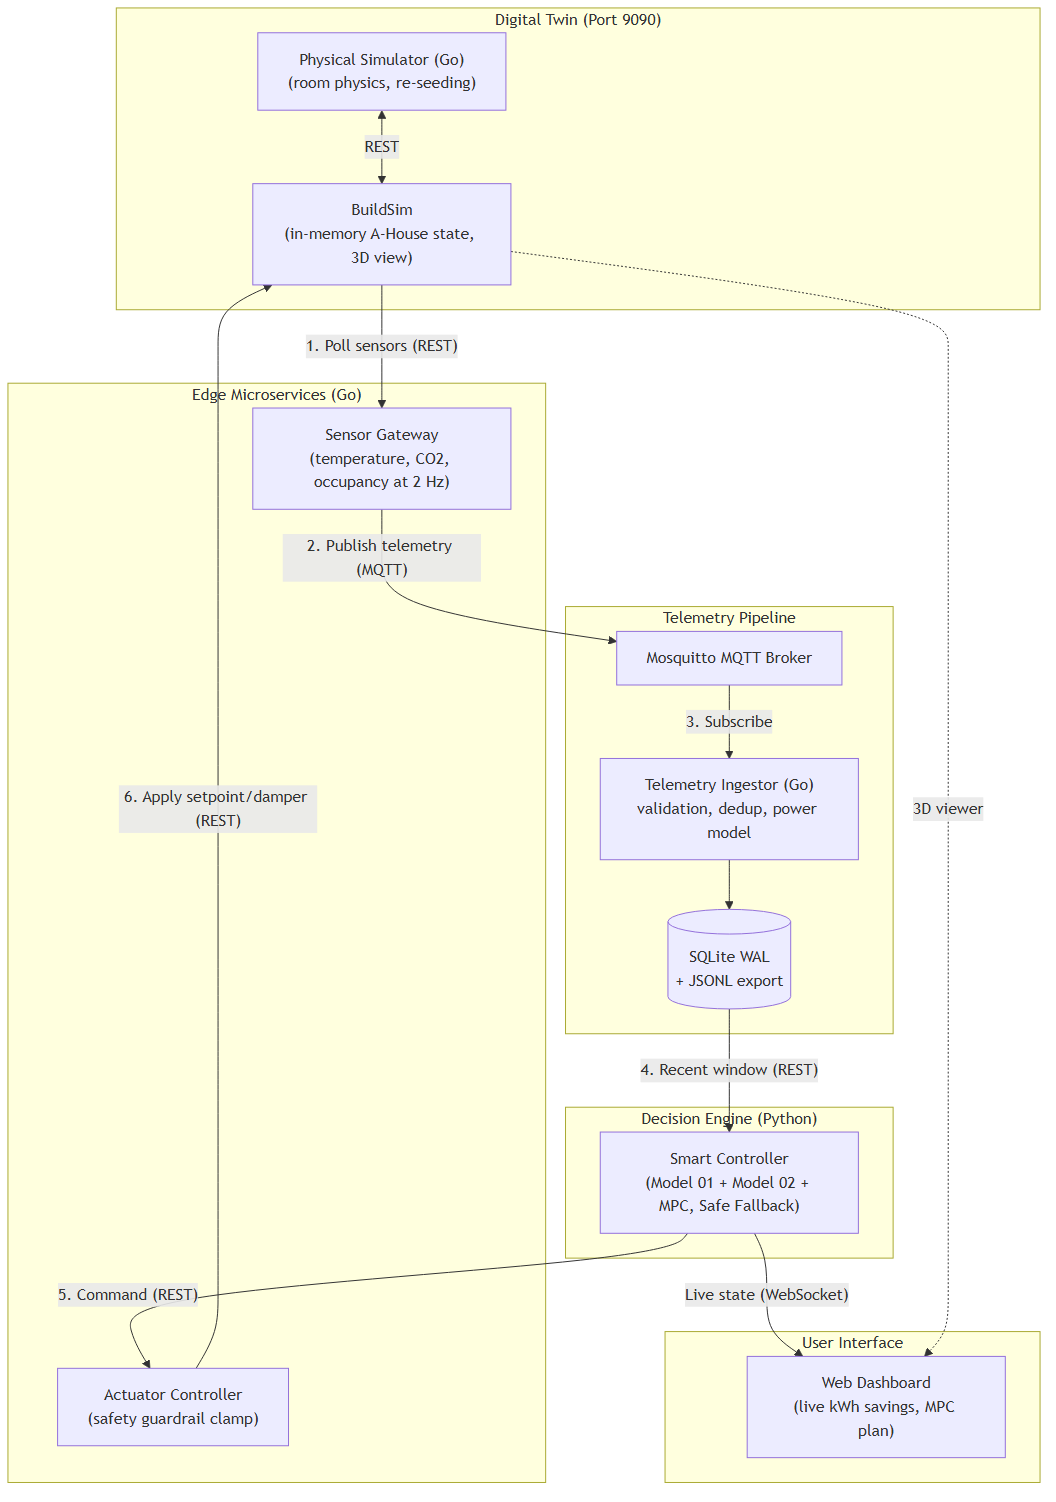
\includegraphics[width=\linewidth]{figures/system_architecture.png}
\caption{Containers and protocols.}
\label{fig:arch}
\end{figure}
Fig.~\ref{fig:arch} shows the eight containers. The Go \texttt{sensor-gateway} polls BuildSim at 2~Hz and publishes to Mosquitto (QoS~0), forwarding each sensor's own timestamp. The Go \texttt{telemetry-ingestor} rejects incomplete bundles and implausible values (temperature outside $-20$--60\degC, \cotwo{} outside 300--5000~ppm, occupancy outside 0--200), stores a row only when the sensor timestamp advanced (so a frozen simulator produces no rows), reads the live setpoint and damper from BuildSim for every row, computes power from them, and writes SQLite in WAL mode. Energy integrates power over the real time between rows. The Python \texttt{smart-controller} hosts the models, the MPC, Safe Fallback and a fixed-schedule baseline twin; the Go \texttt{actuator-controller} is the safety guardrail; a static dashboard shows live state.

\section{Learned Models}
\subsection{Model 01: Occupancy Forecaster}
A Random Forest regressor (60 trees, depth 14) predicts occupancy 5--30~min ahead from local-time calendar features of the target time (hour, weekday, LTU lecture block, lunch, fika), lead time and current occupancy. It is trained on an 8-week synthetic LTU timetable simulated in 5-minute slots with per-lecture attendance, 15\% cancellations and evening study groups; labels are the occupancy observed at $t+$lead. On a chronological hold-out (96 768 samples) it reaches R\textsuperscript{2}~=~0.955 and RMSE 1.26 persons versus 3.60 for persistence; on the unseen benchmark week its 10--30~min MAE is 1.05 persons.

\subsection{Model 02: Thermal and \cotwo{} Predictor}
Two gradient-boosted tree ensembles predict the change in temperature and \cotwo{} over a step from physics-informed features (state, action, occupancy, heating lift, envelope and ventilation drivers, step length). Training combines 4 516 transitions extracted from logged telemetry with 20 000 transitions simulated from the room equations. Held-out R\textsuperscript{2} is 0.9967 for temperature (RMSE 0.26\degC) and 0.9993 for \cotwo{} (RMSE 13.7~ppm). Power is derived from the predicted trajectory by an energy balance rather than learned. Most training data is synthetic, which makes these figures optimistic.

\section{Model Predictive Control and Safety}
\begin{figure}[t]
\centering
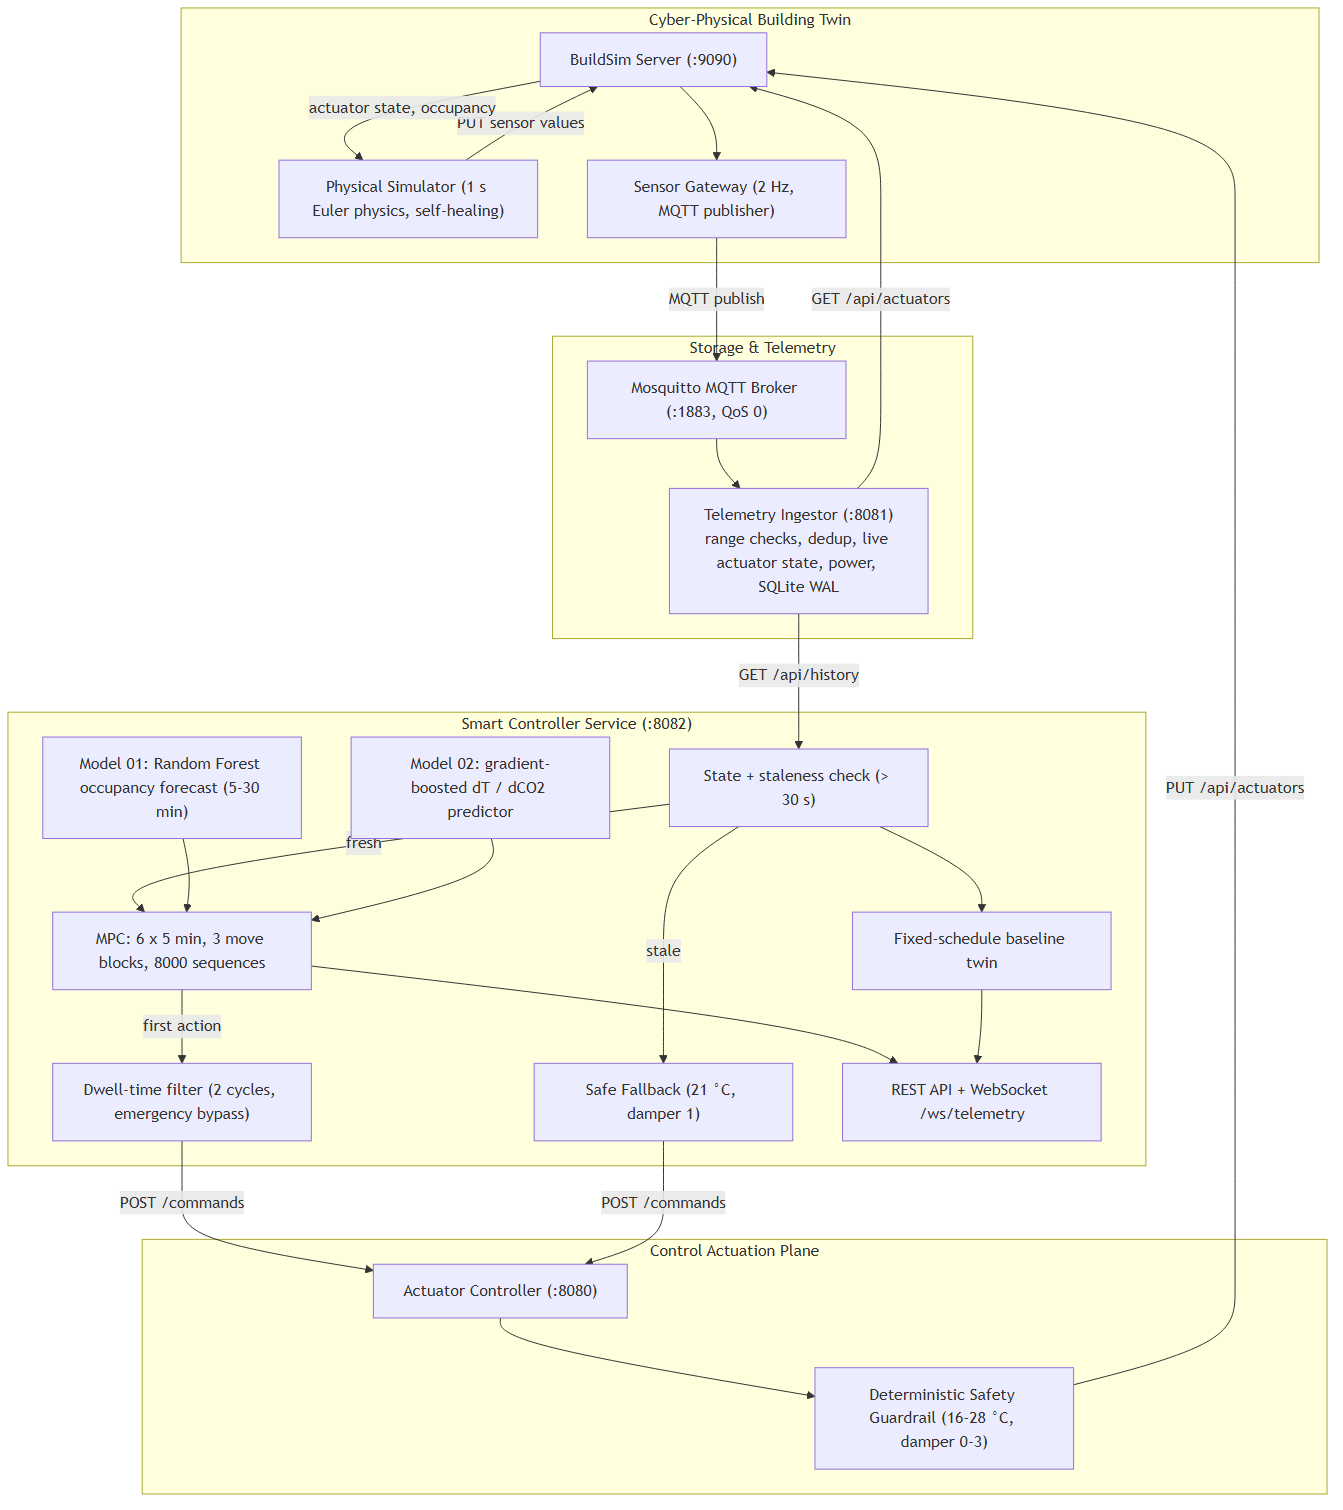
\includegraphics[width=\linewidth]{figures/phase3_mpc_architecture.png}
\caption{Decision path from telemetry to actuators.}
\label{fig:mpc}
\end{figure}
Every 10~s the controller solves a problem over six 5-minute steps (Fig.~\ref{fig:mpc}). Actions are $T_{set}\in\{18,19.5,20.5,21.5,22.5\}$\degC{} $\times$ $D\in\{0,\dots,3\}$. With move blocking the action may change at three block starts (default steps 1, 2 and 4; the third block is aligned with the first forecast occupied/empty transition), giving $20^3=8000$ sequences rolled out through Model~02 in vectorised batches (mean 215~ms, p95 289~ms). Step~1 uses the larger of measured and forecast occupancy; later steps use Model~01. With $\Delta t_h=5/60$~h the cost is
\begin{multline}
J=\sum_{k=1}^{6}\Big[w_e \tfrac{P_k}{1000} + \mathbb{1}_{occ,k}\big(w_T (T_k-21.5)^2 + w_B v(T_k)^2 \\
+ w_C\big(\tfrac{(C_k-800)^+}{100}\big)^2 + w_{C2}\big(\tfrac{(C_k-1000)^+}{100}\big)^2\big) \\
+ (1-\mathbb{1}_{occ,k})\,w_B\,((16-T_k)^+)^2\Big]\Delta t_h + \sum_{\text{blocks}}\big(w_\Delta \Delta T_{set}^2 + w_D|\Delta D|\big)
\end{multline}
where $v(T)$ is the distance outside 20--24\degC, $w_e=1$, $w_T=0.5$, $w_B=20$, $w_C=0.5$, $w_{C2}=10$, $w_\Delta=0.002$ and $w_D=0.005$. The switching weights are small on purpose: an earlier, larger switching cost exceeded the one-step benefit of any damper change and locked the damper at its maximum in an empty room; a regression test now covers this.

A dwell-time filter holds an action change for two control cycles (20~s) unless \cotwo{} exceeds 1100~ppm or an occupied room is below 18\degC. If the newest telemetry row is older than 30~s, the MPC is skipped and the controller commands 21\degC{} with damper~1 (Safe Fallback). The actuator controller clamps setpoints to 16--28\degC{} and the damper to 0--3 and rejects unknown rooms; it is a static guardrail, not a verified runtime-assurance (Simplex~\cite{sha2001using}) architecture.

\section{Communication Protocols}
MQTT~\cite{mqtt5} fans telemetry out from the gateway without coupling it to consumers; at QoS~0, readings published during a broker outage are lost, which is acceptable for 1~Hz state that is superseded a second later. Commands use REST~\cite{fielding2000architectural} because the controller needs an immediate explicit outcome (200 applied, 400 rejected, 502 BuildSim error) and setting a state is idempotent. The dashboard receives pushed state over WebSocket~\cite{rfc6455} (\texttt{/ws/telemetry}), which browsers support natively; MQTT in the browser would need an MQTT-over-WebSocket listener and a client library, and Server-Sent Events would suffice for one-way push but not for future operator commands on the same channel. The dashboard reconnects with exponential back-off and polls REST while disconnected.

\section{Evaluation}
\subsection{Simulated Work Week}
A Monday--Friday timetable drawn with a seed unseen by Model~01 (occupied 31.9\% of the time, peak 24 people) drives four controllers on identical physics, acting every 5~minutes: (1) fixed schedule, 22\degC/damper~2 from 06:00--22:00 and 16\degC/damper~0 otherwise; (2) rule-based, 21.5\degC/damper~2 when occupied and 18\degC/damper~0 when empty; (3) rule-based with demand-controlled ventilation (DCV), damper from measured \cotwo{}; (4) the MPC.

\begin{table}[t]
\caption{Simulated work week (38.3 occupied hours)}
\label{tab:week}
\centering
\begin{tabular}{@{}lrrrr@{}}
\toprule
 & Fixed & Rule & Rule+DCV & MPC \\ \midrule
Energy (kWh) & 112.7 & 44.0 & 47.7 & 52.1 \\
\quad occupied & 23.4 & 20.7 & 24.4 & 26.8 \\
\quad empty & 89.3 & 23.3 & 23.3 & 25.2 \\
In 20--24\degC{} (\%) & 100.0 & 99.7 & 99.7 & 99.8 \\
\cotwo{} $>$1000 ppm (\%) & 27.9 & 27.9 & 12.7 & 0.2 \\
\cotwo{} $>$800 ppm (\%) & 71.4 & 71.4 & 70.5 & 80.8 \\
Action changes & 10 & 46 & 321 & 231 \\ \bottomrule
\end{tabular}
\end{table}

Table~\ref{tab:week} shows that the MPC used 53.8\% less energy than the fixed schedule, almost entirely during empty periods (71.8\% less); while occupied it used 14.7\% more, ventilating to stay under 1000~ppm. It spent only 0.2\% of occupied time above 1000~ppm, far less than any other controller. The occupancy-reactive rules used less energy (the MPC used 18.4\% more than the rule-based controller and 9.1\% more than DCV) but exceeded the \cotwo{} limit for 27.9\% and 12.7\% of occupied time. Most of the saving against the fixed schedule therefore comes from occupancy awareness itself. The MPC spent 99.8\% of occupied time in the comfort band and changed actions 231 times.

\subsection{Live Closed Loop}
An end-to-end test injects 10 people into A109 via BuildSim and checks that the MPC leaves eco setback within 45~s, that ingested rows carry the applied actuator state, and that one minute later the room is within 20--24\degC{} and below 1000~ppm. In the final run the MPC commanded 21.5\degC{}/damper~2 after 11~s, citing a predicted 21.4\degC{} and 707~ppm five minutes ahead; one minute later the room measured 21.3\degC{} and 847~ppm.

\subsection{Fault Injection}
\begin{table}[t]
\caption{Fault injection results}
\label{tab:faults}
\centering
\begin{tabular}{@{}p{0.36\linewidth}p{0.36\linewidth}r@{}}
\toprule
Fault & Behaviour & Recovery \\ \midrule
MQTT broker restart & Clients reconnect; QoS~0 readings during the outage lost & 1.1~s \\
BuildSim restart (state wipe) & Watchdog re-registers A109, telemetry resumes & 3.8~s \\
Commands of 48 and 4\degC & Clamped to 28 and 16\degC & immediate \\
Physics simulator stopped & Safe Fallback after 37.4~s & 10.0~s \\
Controller process exit & Docker restarts it; actuators hold & 7.6~s \\ \bottomrule
\end{tabular}
\end{table}
Table~\ref{tab:faults} summarises \texttt{scripts/test\_resilience.py}. BuildSim recovery depends on the watchdog's 15~s period and varied between runs. Go and Python unit tests (18 Python tests) cover the guardrail, ingestor validation and power model, SQLite migration, physics, MPC behaviour, both models and staleness detection.

\section{Limitations and Future Work}\label{sec:limits}
(1) A single room with time-compressed dynamics: heating just in time costs almost the same as pre-heating, so occupancy forecasts mainly help ventilation; realistic time constants and multi-zone coupling would make prediction more valuable. (2) Both models are trained mostly on synthetic data from the same equations used for evaluation. (3) Constant outdoor temperature and no solar gains. (4) No ventilation heat recovery, which makes ventilation unusually expensive. (5) QoS~0 telemetry. (6) The guardrail is a static clamp. (7) The MPC switches actions often; a real installation needs a longer dwell time or stronger switching penalty. Relative to the proposal, multi-zone control, humidity sensing, a Parquet pipeline (replaced by SQLite with JSONL export) and dashboard heatmaps were not implemented.

\section{Conclusion}
The system closes a sense--reason--act loop across eight containers, forecasts occupancy, predicts the room's response, optimises over 30 minutes, enforces safety limits, detects stale data and recovers from injected faults without intervention. It cut energy by 53.8\% against a fixed schedule and kept \cotwo{} above 1000~ppm for only 0.2\% of occupied time, while simpler occupancy-reactive rules used less energy at the cost of air quality. The value of predictive control depends on the room's time constants and on the chosen energy--air-quality trade-off, and a fair evaluation needs baselines stronger than a fixed schedule.

\bibliographystyle{IEEEtran}
\bibliography{references}

\end{document}
